\section{The comparison morphism} \label{Section comparison morphism}

We summarise the existence of the comparison morphism for $\PP^r$ and how it implies that GW and quasimap invariants of projective space coincide. This has been proven in \cite[Theorem 3]{MOP} and \cite[Section 4.3]{Manolache-Push} (but see also \cite[Proposition 4.1]{Bertram} and \cite[Theorem 7.1]{Popa-Roth} for inspiration). We shall try to clarify as many details as possible, for our own benefit and, hopefully, that of the novice reader.

In order to give a morphism $\comp\colon\M{g}{n}{\PP^r}{d}\to\Q{g}{n}{\PP^r}{d}$ we need to be able to canonically associate a family of quasimaps on a base $S$ to any family of stable maps on the same base.

The pointwise construction is the following: a stable map has no base points, so the only thing that might prevent it from being a stable quasimap is the presence of rational tails (of positive degree, by the stable maps stability condition). Let $C=C^{(0)}\sqcup_{q_i}R_i$ be the source curve; the rational tail $R_i$ has degree $d_i$ and is joined to the permanent curve $C^{(0)}$ at the node $q_i$, which is the only special point on $R_i$; hence all the markings belong to $C^{(0)}$. The map to $\PP^r$ is equivalent to the data of a line bundle $L=f^*\mathcal O_{\PP^r}(1)$ on $C$ and $r+1$ sections $s_0,\ldots,s_r$ thereof. We associate to such a stable map the quasimap $\left(C^{(0)},\mathbf x; L_{|C^{(0)}}\otimes\mathcal O_{C^{(0)}}(\sum_{i}d_iq_i);\hat s_0,\ldots,\hat s_r\right)$, where $\hat s_j$ is the restriction of $s_j$ to $C^{(0)}$, seen as a section of $L_{|C^{(0)}}\otimes\mathcal O_{|C^{(0)}}(\sum_{i}d_iq_i)$ through the inclusion $L_{|C^{(0)}}\hookrightarrow L_{|C^{(0)}}\otimes\mathcal O_{C^{(0)}}(\sum_{i}d_iq_i)$. Notice that the resulting quasimap has a base-point of order $d_i$ at $q_i$.

The construction in families requires us to find a line bundle on the universal curve that is trivial on the rational tails and relatively ample elsewhere. This can be performed at the level of Picard stacks: let $\mathfrak{Pic}_{g,n}^{d,\text{st}}$ be the open substack of $\mathfrak{Pic}(\pi\colon\mathfrak{C}_{g,n}\to\mathfrak{M}_{g,n})$ obtained by requiring that the total degree of the line bundle is $d$, the multi-degree is nonnegative and $\mathcal L\otimes\omega_{\pi}^{\text{log}}$ is ample relative to $\pi$, where $\mathcal L$ is the universal line bundle. Let $T^{\delta}$ be the locus in the universal curve over $\mathfrak{Pic}_{g,n}^{d,\text{st}}$ spanned by rational tails on which $\mathcal L$ has degree $\delta$; this is a Cartier divisor by deformation theory and smoothness of the stack $\mathfrak{C}_{\mathfrak{Pic}}$. Notice that $T^{\delta_0}$ and $T^{\delta_1}$ (say $\delta_0<\delta_1$) do intersect in a stratum of codimension 1 in both of them, where the rational tail splits into two rational components, the furthest from $C^{(0)}$ having degree $\delta_0$.

\begin{center}
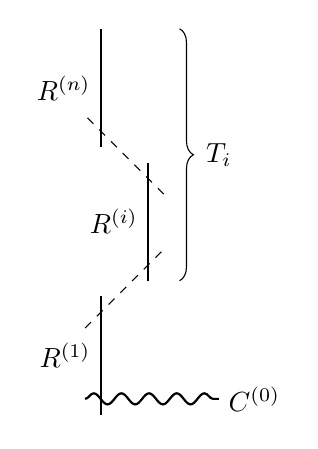
\begin{tikzpicture}
  \draw[thick,decorate,decoration={snake,amplitude=2pt}] (-.2,.2) -- (1.5,.2);
  \node[right] at (1.5,.2) {$C^{(0)}$};
  \draw[thick] (0,0) -- node[left]{$R^{(1)}$} (0,1.5);
  \draw[dashed] (-.2,1.1) -- (.8,2.1);
  \draw[thick] (.6,1.7) -- node[left]{$R^{(i)}$} (.6,3.2);
  \draw[dashed] (.8,2.8) -- (-.2,3.8);
  \draw[thick] (0,3.4) -- node[left]{$R^{(n)}$} (0,4.9);
  \draw [decorate,decoration={brace,amplitude=5pt,mirror}] (1,1.7) -- (1,4.9) node [midway,xshift=.5cm]{$T_i$};
 \end{tikzpicture}
\end{center}

\emph{Claim:} the line bundle $\mathcal M=\mathcal L\otimes\omega_{\pi}^{\text{log}}\otimes\bigotimes_{0<\delta\leq d}\mathcal O_{\mathfrak C}((\delta-1) T^\delta)$ on $\mathfrak{C}_{\mathfrak{Pic}}$ has degree 0 on every component of every rational tail, and is $\pi$-relatively ample elsewhere.

\begin{proof}

Consider a curve $C^{(0)}\sqcup_q R$ with a rational tail of degree $\delta$, such that $R$ consists of $n$ many components $R^{(1)
},\ldots,R^{(n)}$, each of degree $\delta^{(1)},\ldots,\delta^{(n)}$ respectively, numbered from the closest to the farthest from $C^{(0)}$; set $T_i=\bigcup_{j=i}^n R_j$ and $\epsilon_i=\delta-1-\sum_{j=1}^{i-1}\delta_j$.

\begin{center}
\begin{tikzpicture}
 \draw[help lines] (-1,-1) grid (1,1);
 \node[below] at (0,-1) {$T^{\delta_0}$};
 \node[right] at (1,0) {$T^{\delta_1}$};
 
 \draw[gray] (0,-.5) -- (-2,0);
 \draw[decorate,decoration={snake,amplitude=2pt}] (-4,0) -- (-2.5,0);
 \draw (-3.8,-.2) -- node[left]{$\delta_0$} (-3.8,1.3);
 
 \draw[gray] (0,0) -- (-.5,1.5);
 \draw[-,decorate,decoration={snake,amplitude=2pt}] (-1,2) -- (.5,2);
 \draw (-.8,1.8) -- node[left]{$\delta_1-\delta_0$} (-.8,3.3);
 \draw (-1,3) -- node[above]{$\delta_0$} (0.5,3.5);
 
 \draw[gray] (.5,0) -- (2,.5);
 \draw[decorate,decoration={snake,amplitude=2pt}] (2.5,.5) -- (4,.5);
 \draw (2.7,.3) -- node[left]{$\delta_1$} (2.7,1.8);
 
\draw[fill=black] (0,0) circle [radius=1.5pt];
 \draw[fill=black] (0,-.5) circle [radius=1.5pt];
 \draw[fill=black] (.5,0) circle [radius=1.5pt];
 \end{tikzpicture}
\end{center}

A general one-parameter family in $\mathfrak{Pic}_{g,n}^{d,\text{st}}$ will give us a smoothing of such a curve; the universal curve over such a family is a normal surface $S$; we can compute the degree of the restriction of $\mathcal M$ to components of the central fiber of this family by first restricting $\mathcal M$ to $S$, and then using intersection theory on this normal surface.

Notice that restricting $\bigotimes_{0<\delta\leq d}\mathcal O_{\mathfrak C}((\delta-1) T^\delta)$ to this family gives $\mathcal O_S(\sum_{j=1}^n\epsilon_jT_j)$. Since $R^{(i)}$ is a $(-2)$-curve for $i=1,\ldots,n-1$, and $R^{(n)}$ is a $(-1)$-curve, we get

\[
  R^{(i)}.T_j =
  \begin{cases}
    0, & \text{for } j<i \\
    -1, & \text{for } j=i \\
    1, & \text{for } j=i+1 \\
    0 & \text{for } j>i+1 \\
  \end{cases}
\]
hence $\deg(\mathcal M_{|R^{(i)}})=\delta^{(i)}-\epsilon_i+\epsilon_{i+1}=0$ for $i=1\ldots,n-1$, while for $i=n$ it is $\delta^{(n)}-1-\epsilon_n=0$, as $\omega^{\text{log}}$ is trivial on the $(-2)$ curves and has degree $-1$ on $R^{(n)}$. The last assertion of the claim follows from the stability condition and the fact that $O_{\mathfrak C}(T^\delta)$ is effective when restricted to $C^{(0)}$.
\end{proof}

By taking the relative Proj construction we obtain another curve $\hat{\mathfrak C}=\underline\Proj_{\mathfrak{Pic}}\left(\bigoplus_{k\geq 0}\pi_*\mathcal M^{\otimes k}\right)$ over $\mathfrak{Pic}_{g,n}^{d,\text{st}}$, with a map $\rho$ that contracts the rational tails
\bcd
\mathfrak C_{\mathfrak{Pic}}\ar[r,"\rho"]\ar[dr,"\pi"] & \hat{\mathfrak C} \ar[d,"\pi'"]\\
 & \mathfrak{Pic}_{g,n}^{d,\text{st}}
\ecd
It is flat because it is a family of genus $g$ curves over a reduced base. Furthermore, it can be checked by cohomology and base-change \cite[Theorem 12.11]{HAR}\cite[Corollary 1.5]{Knudsen} (notice that the fibers of $\rho$ are either points or rational curves) that $\hat{\mathcal L}=\rho_*\left(\mathcal L\otimes \bigotimes_{0<\delta\leq d}\mathcal O_{\mathfrak C}(\delta T^\delta)\right)$ is a line bundle on $\hat{\mathfrak C}$ of degree $d$ relative to $\pi'$ (such that $\rho^*\hat{\mathcal L}\simeq\mathcal L\otimes \bigotimes_{0<\delta\leq d}\mathcal O_{\mathfrak C}(\delta T^\delta)$), hence the universal property gives us a commutative diagram (with Cartesian square)
\bcd
\mathfrak C_{\mathfrak{Pic}}\ar[r,"\rho"]\ar[dr,"\pi"] & \hat{\mathfrak C} \ar[d,"\pi'"]\ar[dr,phantom,"\square"]\ar[r] & \mathfrak C_{\mathfrak{Pic}}\ar[d,"\pi"] \\
 & \mathfrak{Pic}_{g,n}^{d,\text{st}}\ar[r,"\comp '"] & \mathfrak{Pic}_{g,n}^{d,\text{st}}
\ecd
The very same construction, with the line bundles pulled back from the Picard stack, and the sections of $\mathcal L$ seen as sections of $\mathcal L\otimes \bigotimes_{0<\delta\leq d}\mathcal O_{\mathfrak C}(\delta T^\delta)$ through the inclusion of line bundles ($\mathcal O_{\mathfrak C}(T^\delta)$ is effective), and descended to sections of $\hat{\mathcal L}$ on $\hat{\mathfrak C}$ gives us the comparison morphism $\comp\colon \M{g}{n}{\PP^r}{d}\to\Q{g}{n}{\PP^r}{d}$, fitting in a commutative diagram
\bcd
\M{g}{n}{\PP^r}{d} \ar[d,"\nu_{\mathcal M}"]\ar[r,"\comp"] & \Q{g}{n}{\PP^r}{d}\ar[d,"\nu_{\mathcal Q}"] \\
\mathfrak{Pic}_{g,n}^{d,\text{st}}\ar[r,"\comp '"] & \mathfrak{Pic}_{g,n}^{d,\text{st}}
\ecd
and, as before,
\bcd
\mathcal C_{\mathcal M}\ar[r,"\rho"]\ar[dr,"\pi_{\mathcal M}"] & \hat{\mathcal C}=\comp^*\mathcal C_{\mathcal Q} \ar[d,"\hat\pi"]\ar[dr,phantom,"\square"]\ar[r] & \mathcal C_{\mathcal Q}\ar[d,"\pi_{\mathcal Q}"] \\
 & \M{g}{n}{\PP^r}{d}\ar[r,"\comp"] & \Q{g}{n}{\PP^r}{d}
\ecd

The comparison between virtual fundamental classes is best outlined in the arXiv version of \cite[Remark 5.20]{Manolache-Push}. Call $\nu_{\mathcal M}'=\comp'\circ\nu_{\mathcal M}$. We may endow it with an obstruction theory by means of
\bcd
\nu_\mathcal M^*\mathbf L_{\comp'}\ar[d]\ar[r] & \mathbf E_{\nu'_\mathcal M} \ar[d]\ar[r] & \mathbf E_{\nu_\mathcal M} \ar[d]\ar[r,"{[1]}"] & {}\\
\nu_\mathcal M^*\mathbf L_{\comp'}\ar[r] & \mathbf L_{\nu'_\mathcal M} \ar[r] & \mathbf L_{\nu_\mathcal M} \ar[r,"{[1]}"] & {}
\ecd

Notice that $\comp'$ is a morphism (not of DM type) between smooth Artin stacks, hence we can only deduce that $\mathbf L_{\comp'}$ is supported in $[-1,1]$. It is therefore easily seen that $\mathbf E_{\nu'_\mathcal M}$ is also supported in $[-1,1]$; in order to show that it is actually a perfect obstruction theory, consider the long exact sequence
\begin{align*}
 0 &\to h^{-1}\nu_\mathcal M^*\mathbf L_{\comp'}\to h^{-1}\mathbf E_{\nu'_\mathcal M} \to h^{-1}\mathbf E_{\nu_\mathcal M} \\
 &\to h^{0}\nu_\mathcal M^*\mathbf L_{\comp'}\to h^{0}\mathbf E_{\nu'_\mathcal M} \to h^{0}\mathbf E_{\nu_\mathcal M} \\
 &\to h^{1}\nu_\mathcal M^*\mathbf L_{\comp'}\to h^{1}\mathbf E_{\nu'_\mathcal M} \to 0
\end{align*}
and observe that, dually, $h^{-1}\nu_\mathcal M^*\mathbf T_{\comp'}$ injects into $h^{0}\mathbf E^\vee_{\nu_\mathcal M}\simeq h^{0}\mathbf T_{\nu_\mathcal M}$, because every infinitesimal automorphism of the rational tail induces a nontrivial deformation of the stable map (since the degree of the latter is positive on every component of the rational tail); we conclude that $h^{1}\mathbf E_{\nu'_\mathcal M}=0$.

\emph{Claim:} there is a morphism of obstruction theories $\comp^*\mathbf E_{\nu_\mathcal Q}\to\mathbf E_{\nu_\mathcal M}$ \cite[Lemma 4.19]{Manolache-Push}.

Dually, $\mathbf E^\vee_{\nu_\mathcal M}=R^\bullet\pi_{\mathcal{M}*}\mathcal L^{\oplus r+1}=R^\bullet\hat\pi_*(\rho_*\mathcal L^{\oplus r+1})$, while, by cohomology and base-change, $\comp^*\mathbf E^\vee_{\nu_\mathcal Q}=R^\bullet\hat\pi_*(\hat{\mathcal L}^{\oplus r+1})$, where $\hat{\mathcal L}=\rho_*\left(\mathcal L\otimes \bigotimes_{0<\delta\leq d}\mathcal O_{\mathfrak C}(\delta T^\delta)\right)$, so $\mathbf E^\vee_{\nu_\mathcal M}\to\comp^*\mathbf E^\vee_{\nu_\mathcal Q}$ comes from the inclusion of line bundles on $\mathcal C_\mathcal M$
\[
\mathcal L\hookrightarrow \mathcal L\otimes \bigotimes_{0<\delta\leq d}\mathcal O_{\mathfrak C}(\delta T^\delta).
\]

\emph{Claim:} this morphism factors through $\mathbf E_{\nu'_\mathcal M}$.

\bcd
& \comp^*\mathbf E_{\nu_\mathcal Q}\ar[dl,dashed,"\exists ?"]\ar[d]\ar[dr,"\phi"] & \\
\mathbf E_{\nu'_\mathcal M} \ar[r] & \mathbf E_{\nu_\mathcal M}\ar[r] & \nu_\mathcal M^*\mathbf L_{\comp'}[1]
\ecd

In order to prove that the dashed arrow exists, we need to show that $\phi$ is the zero map. 

This follows formally from the following factorisation:

\bcd
 & & \mathbf L_\comp \ar[ld,"{[1]}" swap] & & \\
\comp^* \mathbf E_{\nu_\mathcal Q}\ar[dd]\ar[r] & \comp^*\mathbf L_{\nu_\mathcal Q}\ar[rr] &  & \mathbf L_{\nu'_\mathcal M}\ar[ul]\ar[dd] & \\
 & & & & \nu_{\mathcal M}^*\mathbf L_{\comp '}[1]\ar[ul,"{[1]}" swap] \\
\mathbf E_{\nu_\mathcal M} \ar[rrr] & & & \mathbf L_{\nu_\mathcal M}\ar[ur] & {}
\ecd

\begin{comment}

\begin{center}

\begin{tikzcd}[execute at end picture={
    \begin{scope}[on background layer]
    \fill[pattern=north east lines, pattern color=gray!20] (a.north west) -- (b.north east) -- (b.south east) -- (a.south west) -- cycle;
    \fill[pattern=north west lines, pattern color=gray!20] (c.north west) -- (c.north east) -- (d.south east) -- (d.south west) -- cycle;
    \end{scope}
  }]
\comp^* \mathbb E_{\nu_\mathcal Q}\ar[d]\ar[r] & |[alias=a]| \comp^*\mathbb L_{\nu_\mathcal Q}\ar[r] & |[alias=c]|\mathbb L_{\nu'_\mathcal M}\ar[r]\ar[d] & |[alias=b]| \mathbb L_\comp \\
\mathbb E_{\nu_\mathcal M} \ar[rr] & & \mathbb L_{\nu_\mathcal M}\ar[d] & \\
 & & |[alias=d]| \nu_{\mathcal M}^*\mathbb L_{\comp '}[1]
\end{tikzcd}

\end{center} 
\end{comment}

\begin{comment}
Dually, we look at $\nu_\mathcal M^*\mathbb T_{\comp'}[-1]\xrightarrow{\phi^\vee} R^\bullet\hat\pi_*(\hat{\mathcal L}^{\oplus r+1})$. Notation: call $R$ the rational tail, joined at the rest of the curve (which we denote by $(C^{(0)},\mathbf p)$ as a marked curve), at the node $q$, which we may occasionally think of as a (smooth) point on $C^{(0)}$. We claim that:
\begin{itemize}
 \item $h^0(\phi^\vee)$ is zero because: the LHS involves automorphisms of the rational tail that leave $C^{(0)}$ fixed, while the RHS involves deformations of $C^{(0)}$, so there is no possible interference.
 \item $h^1(\phi^\vee)$ is zero because: \textcolor{red}{this is slightly awkward.} There are two types of possible contributions to the LHS. They correspond to either moving the node $q$ along $C^{(0)}$, or smoothing it. The former appears in the relative tangent of $\chi'$ only if the marked curve $(C^{(0)},\mathbf p)$ has no automorphisms that may ``move $q$ back'', i.e. $(C^{(0)},\mathbf p)$ is a stable pointed curve. The latter matters only if $(C^{(0)},q,\mathbf p)$ has no moduli, i.e. $(C^{(0)},\mathbf p)$ is a rational tail with less than 3 markings. \textcolor{red}{I will try to justify why the first type vanishes under $h^1(\phi^\vee)$, and leave the second type because I do not understand it as yet.} Look at the long exact sequence
 
\begin{align*}
  0 &\to \Hom(\Omega_{C^{(0)}},\mathcal O_{C^{(0)}}(-q-\sum p_i)) &\to \Hom(\Omega_{C^{(0)}},\mathcal O_{C^{(0)}}(-\sum p_i)) &\to \\
  T_{C^{(0)},q} &\to \Ext^1(\Omega_{C^{(0)}},\mathcal O_{C^{(0)}}(-q-\sum p_i)) &\to \Ext^1(\Omega_{C^{(0)}},\mathcal O_{C^{(0)}}(-\sum p_i)) &\to 0
 \end{align*}
We are interested in what happens to
\[
 \frac{T_{C^{(0)},q}}{\operatorname{Im}\left( \Hom(\Omega_{C^{(0)}},\mathcal O_{C^{(0)}}(-\sum p_i)) \right)}
\]
under $h^1(\phi^\vee)$. If we can show that $h^1(\phi^\vee)$ factors through $\Ext^1(\Omega_{C^{(0)}},\mathcal O_{C^{(0)}}(-\sum p_i))$ we are in business. Indeed the natural maps
\bcd
\Def_L\ar[d]\ar[r] & \Def_{(C,L)}\ar[d]\ar[r] & \Def_C\ar[d] \\
H^1(\mathcal O_C)\ar[r] & H^1(L^{\oplus r+1})\ar[r] & H^1(f^*T_{\PP^r})
\ecd
show that $h^1(\phi^\vee)$ factors through
\[
\Ext^1(\Omega_{C^{(0)}},\mathcal O_{C^{(0)}}(-q-\sum p_i))\to \Ext^1(\Omega_{C^{(0)}},\mathcal O_{C^{(0)}})\to \Ext^1(f^*\Omega_{\PP^r},\mathcal O_{C^{(0)}})\simeq H^1(f^*T_{\PP^r}).
\]
 \item $h^2(\phi^\vee)$ is zero because: $\mathbb E^\vee_{\nu'_\mathcal M}$ is supported in $[0,1]$.
\end{itemize}
\end{comment}
Now the cone $C(\phi)$ gives an obstruction theory relative to $\comp$. A priori, it is supported in $[-2,0]$. By the octahedral axiom
\begin{center}
 \begin{tikzcd}%[cramped]
  \comp^*\mathbf E_{\nu_\mathcal{Q}} \ar[dd,"\phi"]\ar[rrdd,"\phi'"] & & & & & & \\
& & & & & & \\
\mathbf E_{\nu'_\mathcal{M}}\ar[dd]\ar[rr] & & \mathbf E_{\nu_\mathcal{M}} \ar[rrrr]\ar[dr] & & & & \nu_{\mathcal M}^*\mathbf L_{\comp'}{[1]} \\
& & & C(\phi')\ar[urrr] & & & \\
C(\phi) \ar[urrr] & & & & & & 
 \end{tikzcd}
\end{center}
it is enough to observe that $C(\phi')$ is supported in $[-1,0]$ \cite[Lemma 4.20]{Manolache-Push} and that $\nu_{\mathcal M}^*\mathbf L_{\comp'}{[1]}$ is supported in degrees $[-2,0]$, in order to conclude that $C(\phi)=\mathbf E_{\comp}$ is a perfect obstruction theory. The conclusion that
\[
 \comp_*[\M{g}{n}{\PP^r}{d}]^{\text{vir}}=[\Q{g}{n}{\PP^r}{d}]^{\text{vir}}
\]
follows from the connectedness of $\M{g}{n}{\PP^r}{d}$ \cite{KP} (hence of $\Q{g}{n}{\PP^r}{d}$) and an application of the virtual push-forward theorem \cite[Proposition 4.21]{Manolache-Push}.

We shall now explain with an example the reason why a naive attempt to extend the comparison morphism to a general toric variety fails. The problem in a nutshell is that not all toric divisors are nef: a rational tail contained in a divisor which is not nef may have negative degree $-d$ with respect to the corresponding line bundle; when contracting such a rational tail, we shall take the line bundle $L(-dq)$, but what to do with the sections? We would like to divide them by $z^d$, where $z$ is a local coordinate around $q$, but no condition forces such a divisibility to happen. Otherwise said, there is now an inclusion $L_{|C^{(0)}}(-dq)\hookrightarrow L_{|C^{(0)}}$, but the (restriction of the) given sections of $L$ do not necessarily live in the image of $H^0(C^{(0)},L_{|C^{(0)}}(-dq))\hookrightarrow H^0(C^{(0)},L_{|C^{(0)}})$.

A concrete example is found when looking at the Hirzebruch surface $\mathbb F_1=\operatorname{Bl}_{p}\PP^1$.
\begin{figure}
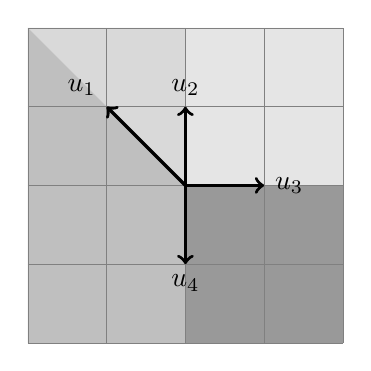
\begin{tikzpicture}
\path [fill=black!10!white] (0,0) -- (2,0) -- (2,2) -- (0,2) -- (0,0);
\path [fill=black!15!white] (0,0) -- (-2,2) -- (0,2) -- (0,0);
\path [fill=black!25!white] (0,0) -- (-2,2) -- (-2,-2) -- (0,-2) -- (0,0);
\path [fill=black!40!white] (0,0) -- (0,-2) -- (2,-2) -- (2,0) -- (0,0);
\draw [help lines] (-2,-2) grid (2,2);
\draw [->,very thick] (0,0) -- (-1,1) node[above left]{$u_1$};
\draw [->,very thick] (0,0) -- (0,1) node[above]{$u_2$};
\draw [->,very thick] (0,0) -- (1,0) node[right]{$u_3$};
\draw [->,very thick] (0,0) -- (0,-1) node[below]{$u_4$};
\end{tikzpicture}
\caption{Toric fan for $\mathbb F_1$.}
\end{figure}

\begin{figure}
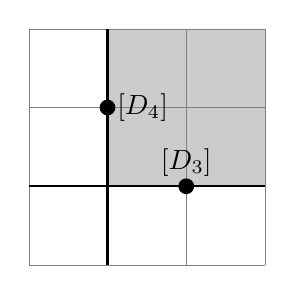
\begin{tikzpicture}
\path [fill=black!20!white] (0,0) -- (2,0) -- (2,2) -- (0,2) -- (0,0);
\draw [help lines] (-1,-1) grid (2,2);
\fill [black] (0,1) circle[radius=.1] node[right]{${[D_4]}$};
\fill [black] (1,0) circle[radius=.1] node[above]{${[D_3]}$};
\draw [thick] (-1,0) -- (2,0);
\draw [thick] (0,-1) -- (0,2);
\end{tikzpicture}
\caption{Nef cone $\operatorname{Nef}(\mathbb F_1)$.}
\end{figure}

\begin{figure}
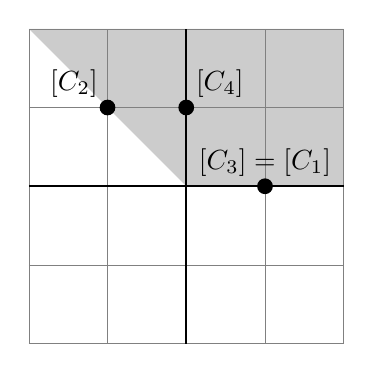
\begin{tikzpicture}
\path [fill=black!20!white] (0,0) -- (2,0) -- (2,2) -- (-2,2) -- (0,0);
\draw [help lines] (-2,-2) grid (2,2);
\fill [black] (0,1) circle[radius=.1] node[above right]{${[C_4]}$};
\fill [black] (1,0) circle[radius=.1] node[above]{${[C_3]}={[C_1]}$};
\fill [black] (-1,1) circle[radius=.1] node[above left]{${[C_2]}$};
\draw [thick] (-2,0) -- (2,0);
\draw [thick] (0,-2) -- (0,2);
\end{tikzpicture}
\caption{Mori cone $\overline{\operatorname{NE}}(\mathbb F_1)$.}
\end{figure}

$\Pic(\mathbb F_1)$ is generated by $[D_3]$ and $[D_4]$, with relations $[D_1]=[D_3]$ and $[D_2]=[D_4]-[D_3]$, and the intersection table is given by
\[
{}
\begin{cases}
 D_3^2=0 \\
 D_3.D_4=0 \\
 D_4^2=1
\end{cases} 
\]
When thinking of $\mathbb F_1$ as a $\PP^1$-bundle over $\PP^1$, $C_1$ and $C_3$ represent the fibers of the bundle (over the toric points of $\PP^1$), while $C_4$ (resp. $C_2$) is the zero/positive (resp. infinity/negative) section; when thinking of $\mathbb F_1$ as $\operatorname{Bl}_{p}\PP^1$, $C_2$ is the exceptional divisor, $C_4$ is the toric line not passing through $p$, and $C_1,C_3$ are the strict transforms of the toric lines through $p$.

Let us look at $\M{0}{2}{\mathbb F_1}{[C_4]}$. Since $[C_4]=[C_2]+[C_3]$, there are going to be maps of the following sort: the source curve is reducible $R_1\sqcup_q R_2$, $R_1$ is mapped isomorphically to a fiber (i.e. in class $[C_3]$) and $R_2$ is mapped isomorphically to $C_2$, all the markings belong to $R_1$. So $R_2$ is a rational tail and deserves to be contracted. Notice that the line bundle $\mathcal O(D_2)$ has degree $-1$ on $R_2$ (and $1$ on $R_1$). In this case everything works well because the corresponding section $u_{2|R_1}$ must vanish at the node, so we can divide it by a chosen (once for all toric line bundles) section of $\mathcal O_{R_1}(q)$.

Consider now $\M{0}{2}{\mathbb F_1}{2[C_2]+[C_3]}$. Certainly there are going to be maps similar to the ones described above, with $R_2$ now covering $C_2$ $2\colon 1$. The point is that $\mathcal O(D_2)$ has degree $-2$ on $R_2$, but $u_{2|R_1}$ doesn't have to vanish at the node of order $2$, so we are in trouble. 
\begin{comment}

\textcolor{blue}{Something is going on here: in this case there is a boundary component where the map is of the type that we have just described, and the requirement that $u_{2|R_1}$ vanishes of order $2$ at the node defines precisely the intersection with the main component. Check this. Could we possibly exploit this phenomenon to define a smaller compactification, possibly even smaller than quasimaps?} 

\end{comment}